\cleardoublepage{}
\chapter{Integrare \texttt{make} negli editor di testo}
\label{cha:editor}

Può essere utile poter richiamare \texttt{make} direttamente dal proprio editor
di testo preferito.  In generale si consiglia di aggiungere il comando
\texttt{make} all'elenco dei comandi di composizione dell'editor, in modo da
poter eseguire la regola predefinita del \texttt{Makefile}.  Di seguito sono
riportate le istruzioni per aggiungere \texttt{make} all'elenco dei programmi di
composizione di alcuni dei più diffusi editor di testo specifici per \LaTeX{}.
Affinché tutti gli editor di testo possano effettuare correttamente l'analisi
dell'output di \texttt{make} è necessario compilare in modalità
\texttt{nonstopmode}.  Questo può essere fatto aggiungendo nel \texttt{Makefile}
ai comandi \texttt{latex} o \texttt{pdflatex} (o l'eventuale altro compilatore
usato) l'opzione \texttt{-interaction=nonstopmode}.
\begin{lstlisting}
# Variabili contenenti i nomi dei comandi da eseguire
# e le relative opzioni.  Per cambiare le opzioni dei
# comandi sarà sufficiente cambiare le variabili
LATEX     = latex -interaction=nonstopmode
PDFLATEX  = pdflatex -interaction=nonstopmode

$(PRINCIPALE_DVI): $(TUTTI_LATEX) immagini-eps
	$(LATEX) $(PRINCIPALE)
	bibtex $(PRINCIPALE)
	makeindex $(PRINCIPALE)
	$(LATEX) $(PRINCIPALE)
	$(LATEX) $(PRINCIPALE)

$(PRINCIPALE_PDF): $(TUTTI_LATEX) $(IMMAGINI_PDF)
	$(PDFLATEX) $(PRINCIPALE)
	bibtex $(PRINCIPALE)
	makeindex $(PRINCIPALE)
	$(PDFLATEX) $(PRINCIPALE)
	$(PDFLATEX) $(PRINCIPALE)
\end{lstlisting}

\section{Emacs}
\label{sec:emacs}

Emacs supporta nativamente \texttt{make}.  È possibile eseguirlo con la
combinazione di tasti \texttt{M-x compile RET} e si può anche specificare la
regola da avviare.  Chi usa il pacchetto AUC\TeX{},
però, potrebbe preferire una migliore integrazione che permetta di effettuare
l'analisi dell'output del programma di compilazione usato.  Per fare ciò bisogna
aggiungere al proprio file di inizializzazione \texttt{.emacs} il seguente
codice
\begin{lstlisting}[language=lisp,morekeywords={eval-after-load,add-to-list}]
(eval-after-load "tex"
  (add-to-list 'TeX-command-list
	       '("Make" "make" TeX-run-TeX nil t)))
\end{lstlisting}
Con questa modifica sarà possibile eseguire \texttt{make} con la combinazione di
tasti \texttt{C-c C-c Make RET}.

\section{Kile}
\label{sec:kile}

Andare nel menu \menu{Impostazioni > Configura Kile}, nella scheda
``Costruzione'', sotto ``Strumenti'', della finestra che verrà aperta, fare clic
sul pulsante \keys{Nuovo\dots{}} sotto l'elenco degli strumenti disponibili.
Nella nuova finestra scrivere ``Make'' nel campo ``Nome dello strumento'', fare
clic sul pulsante \menu{Successivo} e selezionare ``PDFLaTeX'' nel menu a
tendina della classe a cui fare riferimento, quindi fare clic sul pulsante
\menu{Completa}.  A questo punto bisogna configurare lo strumento: nel campo
``Comando'' della scheda ``Generale'' scrivere ``make'', assicurarsi che le
opzioni ``Controlla se il documento radice'' e ``Salta al primo errore'' siano
attive e deselezionare l'opzione ``Esegui automaticamente gli strumenti
aggiuntivi'' (se nei \texttt{Makefile} ci sono già le istruzioni necessaria per
eseguire automaticamente tutti gli eventuali strumenti aggiuntivi).  Nella
scheda ``Avanzate'' assicurarsi che il campo ``Tipo'' sia impostato a ``Esegui
al di fuori di Kile'', il campo ``Classe'' a ``LaTeX'' e il campo ``Stato'' a
``Editor''.  Nella scheda ``Menu'' selezionare ``Compila'' nel menu a tendina
relativo alla voce ``Aggiungi strumento al meno di costruzione'', in questo modo
sarà possibile eseguire \texttt{make} dall'elenco di tutti gli strumenti di
compilazione.

\section{Texmaker}
\label{sec:texmaker}

\begin{figure}
  \centering
  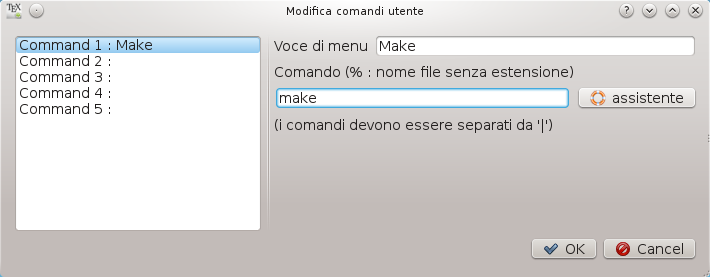
\includegraphics[width=0.8\textwidth]{figure/texmaker}
  \caption{Finestra di configurazione di Texmaker.}
  \label{fig:texmaker}
\end{figure}
Seguendo il menu
\menu{Utente > Comandi personalizzati > Modifica comandi utente} si aprirà una
finestra come quella riportata nella figura~\ref{fig:texmaker} e si deve
scrivere ``Make'' nel campo ``Voce di menu'' e ``make'' nel campo ``Comando''.
In questo modo \texttt{make} sarà eseguibile dall'elenco dei comandi
personalizzati.

\section{TeXstudio}
\label{sec:texstudio}

\begin{figure}
  \centering
  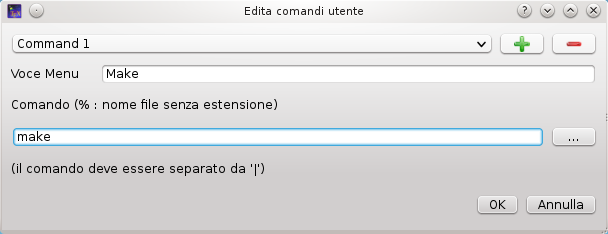
\includegraphics[width=0.8\textwidth]{figure/texstudio}
  \caption{Finestra di configurazione di TeXstudio.}
  \label{fig:texstudio}
\end{figure}
TeXstudio è un fork di Texmaker e la procedura è simile a quella descritta qui
sopra.  Dal menu \menu{Utente > Comandi utente > Edit comandi utente} si aprirà
una finestra come quella riportata nella figura~\ref{fig:texstudio} e nel campo
``Voce menu'' si scriverà ``Make'', nel campo ``Comando'' si scriverà ``make''.
Dopo di ciò sarà possibile eseguire \texttt{make} dall'elenco dei comandi
utente.

\section{Texworks}
\label{sec:texworks}

\begin{figure}
  \centering
  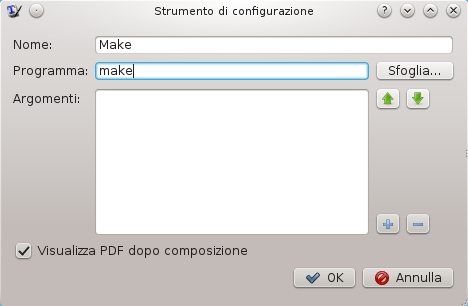
\includegraphics[width=0.8\textwidth]{figure/texworks}
  \caption{Finestra di configurazione di Texworks.}
  \label{fig:texworks}
\end{figure}
Andare nel menu \menu{Modifica > Preferenze} e nella scheda ``Composizione''
della finestra che si aprirà fare clic sul pulsante \keys{{+}} vicino all'elenco
degli strumenti di composizione.  Nella finestra che si aprirà, come quella
riportata nella figura~\ref{fig:texworks}, scrivere ``Make'' nel campo ``Nome''
e ``make'' nel campo ``Programma''.  Dopo di ciò \texttt{make} sarà disponibile
nell'elenco dei programmi di composizione di questo editor di testo.

%%% Local Variables:
%%% mode: latex
%%% TeX-master: "../guidamake"
%%% End:
